\documentclass[review]{elsarticle}
\usepackage{graphicx}
\graphicspath{ {pic/} }
\usepackage{lineno,hyperref}
\usepackage{amsmath}
\usepackage{natbib}
\modulolinenumbers[5]

\journal{Journal of \LaTeX\ Templates}

\bibliographystyle{elsarticle-num}
%%%%%%%%%%%%%%%%%%%%%%%
\newcommand{\dabiaolv}{reach rate }


\begin{document}

\begin{frontmatter}

\title{A data-driven approach for performance prediction for cache group in content delivery network
    %\tnoteref{mytitlenote}
    %JPDC-A data-driven framework for performance evaluation for CDN cache groups
    }
%\tnotetext[mytitlenote]{Fully documented templates are available in the elsarticle package on %\href{http://www.ctan.org/tex-archive/macros/latex/contrib/elsarticle}{CTAN}.}

%% Group authors per affiliation:
\author{None
    %\fnref{myfootnote}
    }
\address{Radarweg 29, Amsterdam}
%\fntext[myfootnote]{Since 1880.}

%% or include affiliations in footnotes:
\author[mymainaddress,mysecondaryaddress]{Elsevier Inc}
\ead[url]{www.elsevier.com}

\author[mysecondaryaddress]{Global Customer Service\corref{mycorrespondingauthor}}
\cortext[mycorrespondingauthor]{Corresponding author}
\ead{support@elsevier.com}

\address[mymainaddress]{1600 John F Kennedy Boulevard, Philadelphia}
\address[mysecondaryaddress]{360 Park Avenue South, New York}

\begin{abstract}
CDN Service providers are increasingly using data-driven mechanisms to build their performance model of their service-providing systems. To build a model to accurately describe the performance of the existing infrastructure is very crucial to make resource management decisions. Conventional approaches that use hand-tuned parameters has its drawback. Recently, data-driven paradigm have been shown to greatly outperform traditional methods in many applications, in both accuracy and their quick reactions to the changing environment. We design a framework that using these techniques to build a performance model. Our approach shows an average 6.98\% improvement in terms of weighted mean absolute percent error (WMAPE) compared to the baseline models.
\end{abstract}
\begin{keyword}
\textit{edge computing, deep learning, content delivery networks, sequence learning, predictive analysis, high dimensional data}
%\texttt{elsarticle.cls}\sep \LaTeX\sep Elsevier \sep template
%\MSC[2010] 00-01\sep  99-00
\end{keyword}
\end{frontmatter}
\linenumbers
\section{Introduction}
% the detail of absract
There is a trend \cite{Jiang2017Pytheas:Exploration-Exploitation} \cite{Mao2017NeuralPensieve} that using data-driven methods to model complex networked systems. Traditional approach typically simple huristics. These methods have several drawbacks  \cite{Mao2017NeuralPensieve}. They cannot quickly respond to the change of the environment. the mothods, changing environment. They cannot accurately reflect and oversimplified the complex systems due to the lack of knowledge of real-word environment. Driven by the opportunity to collect and analyze data (e.g., application quality measurement from end users), many recent proposals have demonstrated the promise of using deep learning to characterize and optimize networked systems. Drawing parralel from the success of deep-learning on pattern recognizaition, instead of using empirical non-linear learning model to descirbe the complex interaction of different features, we use deep learning models and treat networked systems as a black-box.

A content delivery network (CDN) is a globally distributed network system deployed across the Internet. Composed with geographically distributed cache servers, CDNs deliver cached content  to  customers  worldwide  based  on their geographic locations. Extensively  using  cache  servers,  content  delivery over  CDN  has  low  latency  and  high  reliability,  and  supports better quality of experience.

The CDN Service providers are increasingly using data-driven mechanisms to build their performance model of their service-providing systems. To build a model to accurately provice an understanding of the performance of the existing infrastructure such as the health of cache groups and network status, is very crucial to make resource management decisions including content placement, network traffic scheduling, load banlance of the CDN network. 

Generally CDN provicers don't have direct measurement from the clients (the logs from video players, web browser that can show the QoE of clients), so they use the indirect measurement \dabiaolv which is collected from the HA proxy of CDN cache groups. CDN cache group is the one basic unit of CDN infrastrcture. It's slow and expensive, however, for them to collect these measurements. In order to enable themselves make resource manangement decisions in real time, the CDN providers have to use the metrics that can be collected in the real time to infer the \dabiaolv. 

Cache group can be characterised as multi-dimensional, highly non-linear, time variant. The metrics that collected to CDN cache are sequence data that are measured every minute, which have hundreds of dimensions. The state-of-art methods are typically using simple huristics. They are often based on the domian knowledge of operators. 

%Resouoce management involves modeling the status of all available physical resources,based on which to maximize a resource utilization in terms of cost, energy performance\cite{Mistral}, overall profit,etc, and finally request allocation, and workload allocation.
After analysis our problem, we frame out problem as a sequence learning problem, which consists of stages: (1) feature engineering (2) representaion learning by lstm auto-encoder (3) fully connected network/ svm/ other black-box machine learning algorithm to output the predictions. 
%\deep-
lstm,lstm auto encoder and decoder

Our main contributions are listed below:
\begin{itemize}
  \item data-driven approach
  \item performance modeling as sequence modeling problem
  \item anomaly detection(Collective Anomalies a) and prediction
\end{itemize}

first build a prediction model, and then use the prediction model to do the anomaly detection.

The remain organization of this paper is as follows. In Section II, we 
first  introduce the formulation of performance evaluation problem
and  then introduce  our LSTM  based  structure. In Section
III, we introduce reach-rate prediction algorithms based on the
auto-encoder and decoder. In Section IV, we demonstrate
performance  improvements over baseline models. 
Finally, we provide concluding remarks in Section V.
%\cite
\section{Background}
\subsection{CDN related}
\begin{figure}[h]
    \centering
    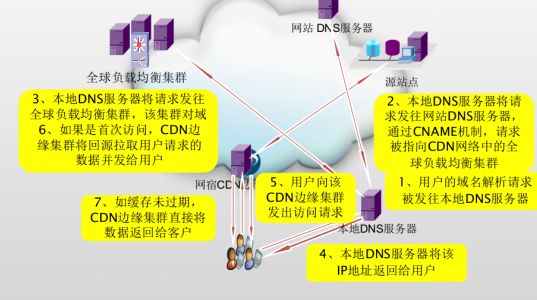
\includegraphics[width=0.5\textwidth]{CDN.png}
    \caption{}
    \label{fig:CDN}
\end{figure}
\begin{figure}[h]
    \centering
    \includegraphics[width=0.5\textwidth]{Cache_group.png}
    \caption{}
    \label{fig:CDN}
\end{figure}
A content delivery network or content distribution network (CDN) is a geographically distributed network of cache servers. CDN helps content provider deliver web pages and other multi-media content to the clients, based on the locations of the clients and cache servers nearby the clients. [CDNs serve a large portion of the Internet content today, including web objects (text, graphics and scripts), downloadable objects (media files, software, documents), applications (e-commerce, portals), live streaming media, on-demand streaming media, and social networks.] CDN play an import role in the internet.

A CDN cache group is a load banlanced cluster that consists of interconnetcted cache servers. ][https://msdn.microsoft.com/en-us/library/ff648960.aspx] The tasks from clients are distributed requests across multiple servers. Load balancers use different algorithms algorithms to maximize the utilization of every server automatically. Round-robin algorithm distributes the load equally to each server. In heterogeneous cluster,  weighted round-robin algorithm is used. A weight was assigned to the server based on its processing capabilities. A heterogeneous cluster adds comlexity to the feature enginnring, as we will discuss in section {}.
\begin{figure}[h]
    \centering
    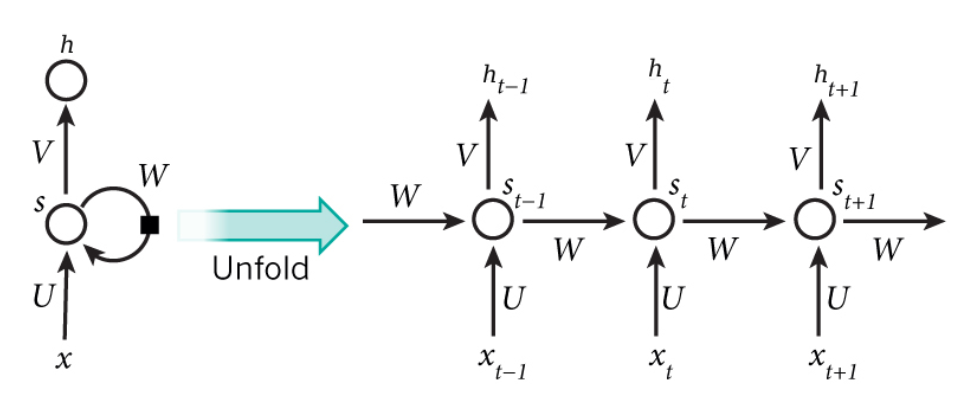
\includegraphics[width=0.5\textwidth]{RNN.png}
    \caption{}
    \label{fig:RNN}
\end{figure}
\subsection{data-driven approach}
In both acdamic and industry,data-driven approach are increasly gaining popularity resulting from the increasing amount of data 
\subsection{Limitations of prior approaches}
\subsubsection{inaccuracy}
  The networked systems are complex and often hard to model accurately. In CDN service deployment disign \cite{}. In cluster scheduling \cite{}, the running time of a task varies with data locality. In automatic bitrate adjustment \cite{Mao2017NeuralPensieve}, the optimal birate depends on the network status.

  Analytical Models are not often accurate enough.

\subsubsection{unable to adapt to the change of the environment}

\section{Problem formulation and Model}
\subsection{\dabiaolv prediction}
\dabiaolv is a indirect measurement of customer QoS
\subsection{Model: performance evaluation problem formulation}
we argue that performance modeling as a sequence learning problem. 
Since we are able to collect the machine performance metrics and network metrics at a certain time interval, we can use a sequence models to describe relationship between machine performances and \dabiaolv
\section{}
There are four catogories of sequence learning problem, which are many to one, many to one and many one. 
Our goal is to predict the future \dabiaolv based on the metrics collected by the monitors. In general, we can use the following formulation to describe the prediction process.
\begin{equation}
	\mathbf y_t = f(x_t,x_t-1,...,x_t-p)
\end{equation}

which is many to one. The training phase is to learn a best function that minimizes the prediction error as follows:
\begin{equation}
	\mathbf h_t = \tanh(\mathbf W * \mathbf h_{t-1} + \mathbf I * \x_t)
\end{equation}

Many models can be used to approximate f in sequence modeling. 

Conventional approaches use AR models. The AR method builds a model of the time series that is composed of a linear part and a random noise part. Whilst the linear part models the ascertainable chunk of the time series, the random noise reflects the unpredictable randomness in the time series. Furthermore, the linear part incorporates l historical values of the time series, which also form the order of the AR model. One commonly refers to the notation AR(l) to indicate how much historical information is used to build the AR model. Equation shows the general autoregressive model for the univariate case. Here, y denotes the time series to be modelled, c denotes the constant parameter of the linear decomposition, β denotes the model to be computed and epsilon reflects the random noise part.

\begin{align}
    y_t = c+\sum_{i=1}^{l}(\beta_i ∗ y_t_−_i)+\epsilon_t
\end{align}


VAR model is a generalization fo AR models. In VAR models, the relationship between the predictor and the target variable is simply described using a linear model as follows: It is used to find a linear model that incorporates the influence of multiple time series into the actual value of a target variable yt.

As such, the equation contains the vectors Yt, Yt−l, the values ?t, c and the model matrices Al. The vectors Yt and Yt−l are composed of all incorporated variables (x, y, z, ...) at time stamp t and t − l. Hence, the i-th element in these vectors is the i-th incorporated variable at the respective time stamps. The matrices A1 . . .Al
reflect the models that need to be fitted. The VAR model is shown in equation 2.21.

\begin{align}
    equation of VAR
\end{align}

Linear models are easy to implement and have good interpretation and thus are widely used in many real work time series analysis problems. However, linear models are shown not sufficient to describe some nonlinear behaviors of the complex network systems. In many cases, neural networks tend to outperform AR-based models [A comparison of artificial neural network and time series models for forecasting commodity prices]. We use deep learning as alternaives.

Deep learning (DL) is a branch of machine learning based on a set of algorithms that attempts to model high-level abstractions in data by using artificial neural network (ANN) ()Figure) architectures composed of multiple non-linear transformations. They have a lot of successful applications in speech and image recognition, machine translation, and forecasting of financial time series. Compared to other machine learning techniques, it can detect complex relationships among features,can extract hierarchical level of features from raw data. So it can produce more accurate result and build a model more with less time.

The essence of DL is to compute hierarchical features or representations of obser-vational data, where the higher-level features or factors are defined from primary lower-level measurements. Based on the features extracted from the data in the training set, the calculations within the model are adjusted so that known inputs produce desired outputs

One of the more popular DL deep neural networks is the Recurrent Neural Network (RNN). RNNs are a class of neural networks that depend on the sequential nature of their input. Such inputs could be text, speech, time series, and anything else in which the occurrence of an element in the sequence is dependent on the elements that appeared before it. .0

\subsection{deep learning in sequence learning}
Sequence prediction often involves forecasting the next value in a real valued sequence or outputting a class label for an input sequence.
\
\subsubsection{RNN}
%The promise of recurrent neural networks is that the temporal dependence and contextual
%information in the input data can be learned.
\cite{Bengio1994LearningDifficult}
\cite{ChoLearningTranslation}

what is RNN and RNN applied in sequence forecast.

\begin{figure}[h]
    \centering
    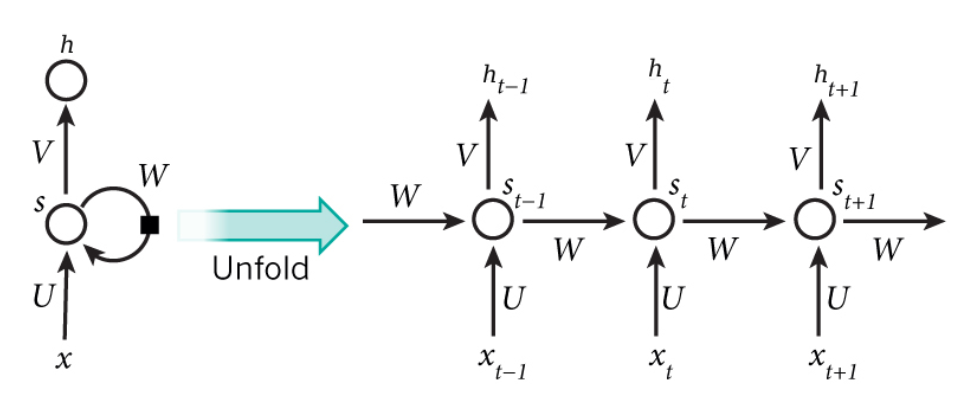
\includegraphics[width=0.5\textwidth]{RNN.png}
    \caption{RNN Architecture}
    \label{fig:RNN}
\end{figure}



\subsection{big data application stack}
spark\cite{ZahariaSpark:Sets};spark streaming\cite{ZahariaDiscretizedClusters};kafka;
\subsection{comparison of exsisting approach}


\subsubsection{our approach}


\section{Methods}
\subsection{Feature Engineering}
The feature enginnering is the process after data-clearsning. The propose of this stage is two-foad:

(1) to find a unified equal-length vector representation of all of the cache groups. 
The metrics collected are in the granuality of machine which have differnet dimensionality. As showed in graph. to make things more complex, a cache group have different vector lengths 

(2) 
\subsubsection{Factors analysis}
(1) specifying the unit of analysis (2) data smurrazation data reduction (3) variable selection (4) 
As there are hundreds of variables, there are many overlaps among the variables. We use correlation in statistis to group highly correlated variables together and create composite measure that can represent each group of variables.

Correlation is an analysis of two or more observed or random variables (except in the special case of auto-correlation 2.2.1) to deter- mine a dependence between the variables. This dependence can be classified as the probability that changes in one variable affect the behaviour of the second variable. The Pearson’s correlation , for instance, defines this dependence in the interval [−1.0, 1.0]. Pearson’s correlation for two given random variables X and Y is computed by dividing the covariance of both variables with the product of their standard deviations.

\begin{equation}
	\mathbf cor_p=p_X_,_Y = \frac{cov(X,Y)}{XY}
\end{equation}

Generally, cases of high correlation compute to a value close to 1.0, high anticorrelation is associated with a value close to -1.0 and no correlation is assumed, if the value is around 0.0. In the last case, the variables appear to be independent. Statistical correlation is used in various domains to identify and better understand relationships of variables. Examples are: medicine, biology, psychology or astronomy

Feature selection: The benefit of this feature selection process is two-fold: (a) a reduced feature set will control the model complexity during model learning, and (b) the processes gain more insights on the complex interaction of different matrics. \cite{Yeom2016Data-DrivenMatrices}. Some Deep Learning algorithms can become prohibitively computationally-expensive when dealing with high-dimensional data. 



\begin{figure}[h]
    \centering
    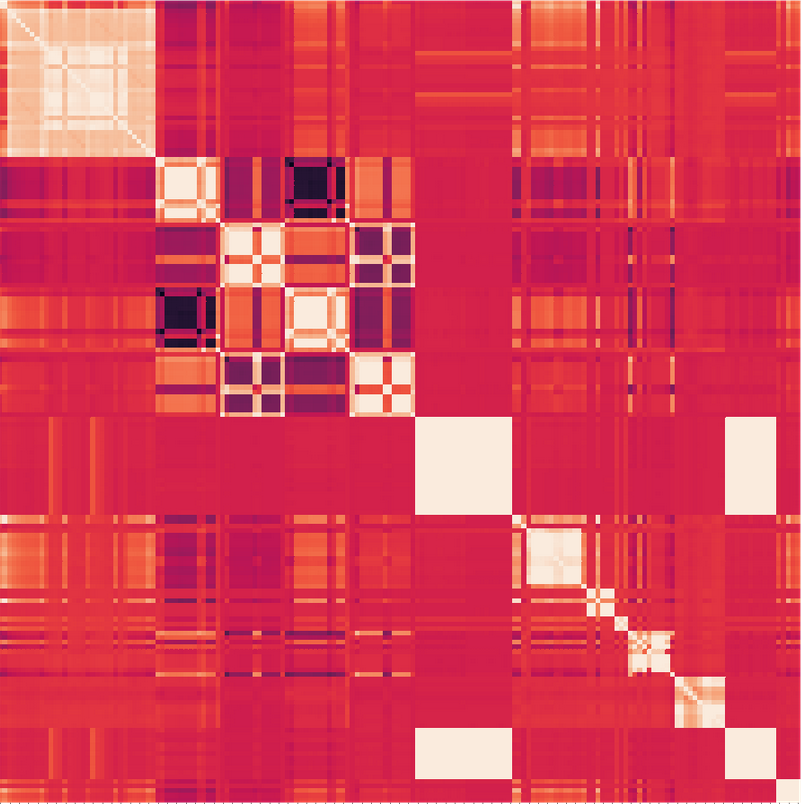
\includegraphics[width=0.5\textwidth]{Correlation_Matric.png}
    \caption{Correlation Matric}
    \label{fig:Correlation Matric}
\end{figure}

\begin{table}[]
\centering
\begin{tabular}{|c|c|}
\hline  
feature &   meaning\\
cpu1.usage &   cpu used ratio of cpu1\\
cpu2.usage &   cpu used ratio of cpu2\\
cpu4.usage &   cpu used ratio of cpu2\\
... & \\
\hline  
mem\_cached & \\
mem\_buffers\_cache\_free & \\
memory.swap  &\\ 
\hline  
channeltraffic\_in   & \\
channeltraffic\_in   & \\
\hline  
disk.used.sda1 &\\
disk.used.sda2 &\\
disk.used.sda3 &\\
\hline  
ioutil\_util\_sda & \\
ioutil\_util\_sdb & \\
ioutil\_util\_sdc & \\
ioutil\_util\_sdd & \\
iowait.wait & \\
\hline
hitratio.port8101 & \\
hitratio.port8102 & \\
\hline        
\end{tabular}
\caption{list of candidate input features from one cahce server,We organize the features into groups}
\label{my-label}
\end{table}



\subsection{Prediction Model Design}
Samples  are  constructed  using  a  sliding  window  with step size one, where each sliding window contains the previous 28 minutes as input, and aims to forecast the upcoming \dabiaolv. the \dabiaolv is stationary ....
\subsubsection{RNN}
RNNs maintain a hidden vector $\mathbf h$, which is updated at time step $t$ as follows:
 
\begin{equation}
	\mathbf h_t = \tanh(\mathbf W * \mathbf h_{t-1} + \mathbf I * \x_t)
\end{equation}

where $\tanh$ is the hyperbolic tangent function, $\mathbf W$ is the recurrent weight matrix and $I$ is a projection matrix. The hidden state $\mathbf h$ is then used to make a prediction

\begin{equation}
	\mathbf y_t = \text{softmax}(\mathbf W * \mathbf h_{t-1})
\end{equation}

where $\textit{softmax}$ provides a normalized probability distribution over the possible classes and $\mathbf W$ is a weight matrix. By using $\mathbf h$ as the input to another RNN, we can stack RNNs, creating deeper architectures \citep{pascanu2013construct}

\begin{equation}
	\mathbf h_t^{l} = \sigma(\mathbf W * \mathbf h_{t-1}^{l} + \mathbf I * \mathbf h_t^{l-1}).
\end{equation}

Training vanilla RNNs is known to be particularly difficult, with vanishing and exploding gradients being one possible explanation \cite{pascanu2012difficulty}.

\subsubsection{RNN encoder-decoder}
\cite{ChoLearningTranslation}
\begin{figure}[h]
    \centering
    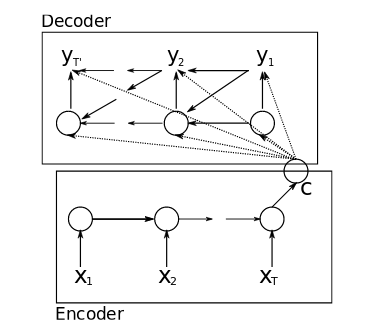
\includegraphics[width=0.5\textwidth]{RNN_encoder-decoder.png}
    \caption{neural network architecture}
    \label{fig:RNN_encoder-decoder}
\end{figure}
applications: machine translation, learning to excute, image captioning, conversational modeling

RNN Encoder-Decoder, consists of two recurrent neural networks (RNN) that act as an encoder and a decoder pair. The encoder maps a variable-length source sequence to a fixed-length vector, and the decoder maps the vector representation back to a variable-length target sequence. \cite{ChoLearningTranslation} also known as sequence embedding. The point of training an autoencoder is to make an RNN learn how to compress a relatively long sequence into a limited, dense vector.

\subsubsection{LSTM}
LSTM, introduced in \cite{Hochreiter1997LongMemory}, addresses the problem of vanishing gradients by introducing a memory cell which ensures constant error flow and gating units. The inner working of LSTM are listed follows:
\begin{equation}
	\begin{split}
		& \mathbf g^u = \sigma(\mathbf W^u * \mathbf h_{t-1} + \mathbf I^u * \x_t) \\
		& \mathbf g^f = \sigma(\mathbf W^f * \mathbf h_{t-1} + \mathbf I^f * \x_t) \\
		& \mathbf g^o = \sigma(\macpu_usage_cpu1thbf W^o * \mathbf h_{t-1} + \mathbf I^o * \x_t) \\
		& \mathbf g^c = \tanh(\mathbf W^c * \mathbf h_{t-1} + \mathbf I^c * \x_t) \\
		& \mathbf m_t = \mathbf g^f \odot \mathbf +  \mathbf g^u \odot \mathbf g^c \\
		& \mathbf h_t = \tanh(\mathbf g^o \odot \mathbf m_{t-1})
	\end{split}
\end{equation}


\subsection{lstm auto-encoder}
Autoencoders are data-specific. Autoencoders are lossy. Autoencoders are learned automatically from data examples, which is a useful property: it means that it is easy to train specialized instances of the algorithm that will perform well on a specific type of input. It doesn't require any new engineering, just appropriate training data. \cite{BuildingKeras}

An autoencoder contains: an encoding function, a decoding function, and a distance function between the amount of information loss between the compressed representation of your data and the decompressed representation (i.e. a "loss" function). The encoder and decoder will be chosen to be parametric functions (typically neural networks), and to be differentiable with respect to the distance function, so the parameters of the encoding/decoding functions can be optimize to minimize the reconstruction loss, using Stochastic Gradient Descent. 

\cite{MalhotraLongSeries} applied in time series. Long Short-Term Memory (LSTM) is able to solve many time series tasks unsolvable. by feedforward networks using fixed size time windows\cite{Gers2001ApplyingApproaches}.

\begin{figure}[h]
    \centering
    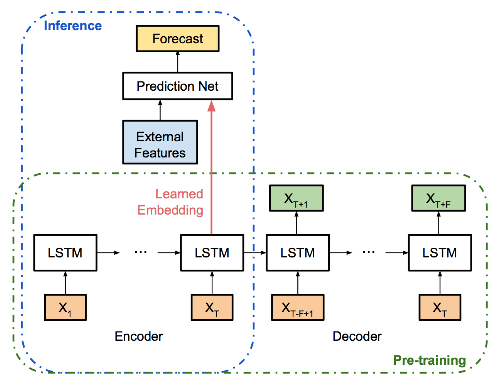
\includegraphics[width=0.5\textwidth]{neural_network_architecture.png}
    \caption{neural network architecture}
    \label{fig:neural_network_architecture}
\end{figure}

Model: We are inspired by ideas of Uber. Prior to fitting the prediction model, we first conduct a pre-training step to fit an encoder that can extract useful and representative embeddings froma  time  series.  The  goals  are  to  ensure  that  (i)  the  learned embedding  provides  useful  features  for  prediction  and  (ii) unusual input can be captured in the embedded space, which will get further propagated to the prediction network in the next step.

As you can see in the figure \ref{fig:neural_network_architecture}, the  function grows near 0. Also, in the page \pageref{fig:neural_network_architecture} 
is the same example.


// how to data clearnsing
// how to construct model

\section{Evaluation}
\subsection{Experimental Settings}
Our implementation using the Google machine learning library, Tensorflow, version 1.2.0. We ran our experiments on a physical machine running an Ubuntu 16.04 imag, interl i7, 8 GB memory, and GPU gtx1060.
The data is collected from the daily operation of CDN cache groups
In this section, we illustrate the model performance using \dabiaolv data collected from a cache group in a selected PoP that provide content caching service for several customers. 

We  use  three  weeks  of  data  as  the  training  set,  the following four  days  as  the  validation  set,  and  the  final three  months  as  the  testing  set.  The  encoder-decoder  is constructed  with  two-layer  LSTM  cells,  with  128  and  32 hidden states, respectively. The prediction network has three fully  connected  layers with tanh activation

The training method we use is mini-batch gradient descent. The hyperparemeter are listed in table.

\subsection{Baseline}
We compare our model with other baseline model which are listed follow:
\begin{enumerate}
  \item ARIMA Model: a naive model that takes last ouput as the prediction
  \item Vanilla LSTM Model
  \item LSTM encoder-decoder with multiple-layers perceptions
  \item LSTM encoder-decoder with multiple-layers perceptions and attention
\end{enumerate}

inally,  Figure   visualizes  the  true  values  and  our predictions during the as an example. We observe that accurate predictions are achieved not only in regular days, but also during holiday seasons.


\subsection{Performance}
\begin{table}[]
\centering
\caption{My caption}
\label{my-label}
\begin{tabular}{lllll}
location & Persistent & LSTM & LSTM encoder-decoder & Our model \\
Shanghai & 10.0       & 9.9  & 8.8                  & 7.7       \\
Shenzhen & 10.0       & 9.9  & 8.8                  & 7.7       \\
Zhejiang & 10.0       & 9.9  & 8.8                  & 7.7      
\end{tabular}
\end{table}

compare four different models in terms of training time and accuracy 

\section{Discussion and Future Work}
A unified models for different cache groups.

further improve accuracy

uncertainty

qualified rate is an indirect measurement;collecting client data.

change detection
\section{Related Work}
When evaluating the's complex system, the evaluation method can fall into three catogory: model-driven method, data-driven method and qualitative knowledge-driven method. The data characterizing the state of system instead of the analytical model is neceessary. In model-drvien method, the mathematical model characterizing the inner 
components of a system has to be all known{\Rethinking_CDN}. When the 
\cite{Jiang2017Pytheas}.\cite{Mao2017NeuralPensieve}.\cite{c}. [From the characteristics of the above methods, the data driven method, which takes the gathered data
as basis and is independent of the object’s prior knowledge, is a more
useful approach for fault prediction and reliability evaluation]l

CDN: two types: long-term, short term;CDN selection \cite{Jiang2017Pytheas:Exploration-Exploitation}

deep-learning; RNN; RNN encoder-decoder; LSTM; LSTM time-series application; LSTM with attention; sequence learning with lstm:
Real-Time Prediction of Taxi Demand Using Recurrent Neural Networks

deep learning and streaming data \cite{Najafabadi2015DeepAnalytics} incremental feature learning and extraction, denoising autoencoders, and deep belief networks

In the operating process of some practical industry systems, the fault
prediction and reliability evaluation technologies can be used to reduce
the cost of system’s maintenance (Wang et al., 2008; Ding et al., 2014;
Alghazzawi and Lennox, 2009). The technologies also can provide reli-
able evidence for system’s repairing opportunity determination, under
this circumstance, the blindness of device maintenance can be reduced,
and the effective time of system running can be greatly increased. Fault
prediction and reliability evaluation, which are important measures
guaranteeing the reliability of system and have received more attention
in recent ten years, are key technologies for complex engineering
systems’ predictive maintenance. According to the difference of the
known condition forms for specific problems, the fault prediction and
reliability evaluation methods fall into three categories: model-driven
method, data-driven method and qualitative knowledge-driven method.
The precondition of model driven method (Isermann, 2005; Si et al.,
2011) is that the mathematical model characterizing the physical laws
of a system has been known. In data-driven method (Jiang et al., 2014;
Wang and Yin, 2014; Mahadevan and Shah, 2009), the analytical model
of system is not required to be known, but the quantitative data samples
characterizing the state of system must be known. The qualitative
knowledge driven method  (Hu et al., 2011) allows the analytical
model to be unknown, but the qualitative knowledge characterizing
the features of system must be gained. From the characterist ics of the
above methods, the data driven method, which takes the gathered data
as basis and is independent of the object’s prior knowledge, is a more
useful approach for fault prediction and reliability evaluation (Hsu et
al., 2010; Chirico and Kolodziej, 2014; Svärd et al., 2014; Si et al., 2012).

As an important direction, the time series analysis and prediction
using some learning algorithms in data-driven fault prediction and
reliability evaluation methods has received widespread attention. On
this basis, some good research results appeared, which mainly focused
on the time series prediction and detection analysis using the intelli-
gent algorithms such as neural networks and support vector machine
(SVM) (Dash et al., 2007; Daewon and Jaewook, 2007; EI-Koujok et al.
Our work:2014). But in practical problems, the state of system is usually decided by multiple correlative factors, so the system being observed is often characterized by multiple correlated variables, the time series observed is commonly called multivariate correlated time series. For this reason, the characters of data must be fully considered in some procedures including the modeling based on system data, monitoring of system state and evaluation of system reliability. While for the above mentioned multivariate time series prediction, many problems can be classified as the modeling category on multi-input multi-output (MIMO) samples, such as fault prediction for MIMO systems, fault forecasting based on multi-step prediction of time series, and so on. The essence of all these problems is seeking for a mapping relationship between the multi-input samples and the multi-output samples. In recent years, the black-box modeling based on input and output data is also a research focus, the relevant techniques gain wide attention and some research findings have emerged. Some effective modeling methods, such as neural network based modeling, wavelet network based modeling, gain much popularity since then. Due to the perfect nonlinear mapping performance and generalization ability, the SVM based on statistical learning theory is introduced to the black-box modeling field and has acquired good effect.
    \cite{Wang2017}

\section{Conclusion}

This paper shows that it is feasible to apply state-of-the-art Deep RL techniques to large-scale networked systems that provides esimation for its performance. The use of . The Using the LSTM encoder-decoder with a full connected  offer a modeling selection for similar problems.
\section*{References}

\bibliographystyle{unsrt}
\bibliography{mendeley}

\end{document}